\documentclass[11pt,a4paper]{article}
\usepackage[utf8]{inputenc}
\usepackage{amsmath}
\usepackage{amsfonts}
\usepackage{amssymb}
\usepackage{graphicx}
\usepackage{algorithm,algpseudocode}



\usepackage{macros/minesu_macro}

\usepackage[left=2cm,right=2cm,top=2cm,bottom=2cm]{geometry}
\title{ Contamination-Aware Experiments on Networks }

\author{
Mine Su Erturk\\
Graduate School of Business\\
Stanford University\\
   \texttt{mserturk@stanford.edu} 
  \and
Eray Turkel\\
Graduate School of Business\\
Stanford University\\
   \texttt{eturkel@stanford.edu} 
}

\date{}
\begin{document}
\maketitle

\section{Introduction}
We study the problem of a decision maker (DM) conducting experiments over time, on a network environment. An `experiment' in the context of our model is treating a node in the network. Each node responds to the treatment differently, depending on their (observable) characteristics. We also assume that treating a node creates spillovers on neighboring nodes. The DM's goal is learning the optimal treatment allocation over the network by sequentially conducting local experiments on different nodes. 

We assume that there are multiple analysts conducting experiments on the network, as is the case in many online platforms. The DM's experiment creates negative externalities on other ongoing experiments, or the deployed treatments from previously run experiments. We model this as a cost for contaminating the treatment regime of other experimenters. Therefore, the DM has to strike a balance between learning the treatment response function efficiently, and staying within acceptable levels of contamination. We analyze the DM's problem as a sequential decision making problem, which puts our framework closer to the literature on online learning and bandits, instead of using a randomization based inference setting, as is common in the network experimentation literature.

\section{Model}

There are N units connected on an undirected, unweighted graph. Denote each unit on the graph by $i \in \{1, \dots, N \}$. The units have observable characteristics, $\{x_1 , \dots, x_N \}$ with $x_i \in \mathbb{R}^k$. The DM's objective depends on the outcomes of the units, denoted $\{Y_1 , \dots, Y_N\}$ with $Y \in \mathbb{R}$, which respond to a treatment regime that will be determined. The decision maker can run experiments sequentially, at time periods $t \in \{1, \dots , T\}$. Let $w_{it}$ denote the treatment assignment for node $i$ during the period of experimentation $t$, with $w_{it} \in \{0,1\}$, and denote the vector of treatment assignments at time $t$ by $w_t = [w_{1t}, \dots , w_{Nt}] \in \{0,1\}^N$. We assume that the experimentation is local, in the sense that every period, only one node can be treated. Thus for all time periods $t$, $\sum_{i \leq N} w_{it} = 1$.

Each node's outcome depends on their characteristics, the treatment they receive and the exposure to the treatment through their neighbors. Define the exposure for node $i$ at period $t$ as $e_{it}$, which is assumed to be: 
$$e_{it} = \frac { \sum_{j \leq N}  \mathbf{1}(j \in nhbd(i)) w_{jt}}{ \sum_{j \leq N} \mathbf{1}(j \in nhbd(i)) }$$

$Y$ is assumed to be a linear function of the unit characteristics and the exposure to the treatment:

$$Y_{it}( w_{it}, e_{it}) = \beta^T x_i + \Gamma^T x_i e_{it} + \epsilon_i,$$

where $\beta, \Gamma \in \mathbb{R}^k$, and for all nodes $i$, $\epsilon_i \sim N(0, \sigma^2_\epsilon)$.

 The DM's goal is to choose a treatment assignment policy over the network based on the value of $\Gamma$. Denote the final treatment assignment for node $i$ by $w_i$, dropping the time subscript. We denote a policy by $\pi(\Gamma)$, where $\pi(\Gamma)=[w_1, \dots , w_N] \in \{0,1\}^N$. We assume that there is an upper limit on the number of nodes that can be treated in the final deployment, which we call $D$, i.e., $\sum_{i \leq N} w_i \leq D$. 

At every period $t$, the DM's experimentation creates a cost, because the experiment interacts with a previous experimenter's treatment allocation, contaminating their results. We assume that the cost is proportional to the number of units exposed to the treatment, and once a unit is exposed, future exposures of that unit do not increase the cost any further. Define the total cost of experimentation at period $t$ by:

$$c_t = c \sum_{i \leq N} \mathbf{1}\left( e_{it} > 0 \mbox{ and } e_{is}=0,  \forall s<t \right) .$$

Throughout, we will let $c=1$ for simplicity. Hence, the total cost incurred through experimentation by the DM can be written as   $C= \sum_{t \leq T} c_t  .$ We assume that the DM has to stay below a `contamination budget' of at most $\bar{C}$ during experimentation. Then, as a function of the contamination budget $\bar{C}$, we define the value of a policy as follows:

$$V(\pi, \bar{C})=\sum_{i \leq N} \Gamma^T x_i e_i(\pi), $$

where $e_i(\pi)$ denotes the exposure function determined at the last period for final deployment, induced by the treatment allocation under policy $\pi$, decided after an experimentation period with the contamination budget $\bar{C}$. The DM does not observe the true vector $\Gamma$ but has an imperfect estimate of it learned through sequential experimentation, which we will call $\hat \Gamma$. The DM maximizes the empirical value function using its estimate at the end of the experimentation period:

\begin{align}\label{eq:dm_opti}
Max_{\hat \pi} : \sum_{i \leq N} \hat \Gamma^T x_i e_i(\hat \pi)  \quad \mbox{s.t. } 1^T \hat \pi \leq D .
\end{align}

\iffalse
This ends up being equivalent to this minimization (the equivalence to be clarified later):
%

$$ Min_{\hat \pi} E \left( Sup_\pi \left(\sum_{i \leq N} \Gamma^T x_i e_i(\pi) - c_\infty(\pi) \right) - \sum_{i \leq N} \hat \Gamma^T x_i e_i(\hat \pi) + c_\infty(\hat \pi) \right) $$
%
OR (depending on how $\hat \Gamma \rightarrow \Gamma$).

$$ Min_{\pi} E \left( Sup_\pi \left(\sum_{i \leq N} \Gamma^T x_i e_i(\pi) - c_\infty \right) - \sum_{i \leq N}  \Gamma^T x_i e_i(\pi) + \hat c_\infty \right) $$
\fi

Let $X_{K \times N}$ denote the matrix of covariates for all the nodes on the graph, and let $X_s$ denote the analogous matrix only for nodes that were exposed to the treatment during the experimentation period. Let $\hat \Gamma _{1 \times K}$ be the vector of estimated coefficients.

Define the vector of exposure values at time t as $\bar e_t=[\mathbf{1}(e_{1t}>0), \dots, \mathbf{1}(e_{Nt}>0)]_{1 \times N}$ and let $c_t$ denote the cost vector at time t.  We can recursively write: $c_0 = 0_{1 \times N}, c_1 = \bar e_1$, and generally, $c_n = (c_{n-1} + \bar e_n) - (Diag(c_{n-1})  \bar e_n) $. $Diag(c_n)$ denotes the diagonal matrix with the entries of $c_n$ on its diagonal entries. This recursive formulation captures the notion that the cost of second and future exposures to the experiment are zero.

We can also define the final exposure vector $e$ in terms of the adjacency matrix of the network, $A_{N \times N}$ (with self-edges), and the final treatment allocation vector $\pi \in \{0,1\}^N$. Representing $e$ as a vector, we have: $Diag(A \mathbf{1}_{N} ) ^{-1} A\pi  = e$, where $\mathbf{1}_{N}$ is an $(N \times 1)$ vector of 1's. Therefore, we can rewrite the maximization problem \eqref{eq:dm_opti} as a convenient linear program, where we relax $\pi_i$ and allow it to take values in $[0,1]$, interpreting the resulting policy as a probabilistic treatment assignment rule:

\begin{align}\label{eq:dm_opti_lin}
Max_{\hat \pi}: \left(\hat \Gamma^T X Diag(A \mathbf{1}_{N} ) ^{-1} A \right) \hat \pi  \textit{, subject to: } 1^T \hat \pi \leq D , \forall i, \hat \pi_i \in [0,1]
\end{align}


%$$Max_{\hat \pi}: E \left( \left(\hat \Gamma^T X Diag(A \mathbf{1}_{N} ) ^{-1} A \right) \hat \pi  -  c_\infty(\hat \pi) \right)$$

\iffalse
or, we can write: %here y captures the cost structure using a linear formulation

$$Max_{\hat \pi, y_i}: E \left( \left(\hat \Gamma^T X Diag(A \mathbf{1}_{N} ) ^{-1} A \right) \hat \pi  - \sum_{i \leq N} y_i \right)$$ subject to: 

$$\forall i,  \left( Diag(A \mathbf{1}_{N} ) ^{-1} A \hat \pi \right)_i \leq y_i$$

$$\forall i, y_i, \hat \pi_i \in \{0,1\} $$
\fi

\section{Regret Analysis}
Let $\hat \pi$ denote the optimal policy maximizing the optimization problem \eqref{eq:dm_opti_lin} given that the DM has estimated the coefficient vector as $\hat{\Gamma} $, which achieves the value $V(\hat \pi, \bar{C})$. Let $V(\pi^*)$ be the optimal value achievable by the oracle who solves the optimization problem \eqref{eq:dm_opti_lin} with the true coefficient vector $\Gamma$. Thus, we can define the regret as follows:

$$R = V(\pi^*) - V(\hat \pi, \bar{C}) .$$

To analyze the regret of the empirical value maximizing policy $\hat \pi$, let us introduce some notation. Let $\sigma_j( A)$ denote the $j^{th}$ eigenvalue of the matrix A, with $\sigma_1$ being the largest. Suppose that the covariate matrices $X, X_s$ are standardized, so the matrix $X X^T$ is the symmetric correlation matrix. 
\begin{thm}
Fix $\tau \geq 0$. Then, regret is bounded above by K with the following probability:
\begin{align}
\bP(R \leq K) \geq 1 - \exp{\lt( -\frac{1}{2} (\tau -1 )^2 \rt)},
\end{align}
where
\begin{align}\label{eq:Kterm}
K =\frac{  \delta  \max \{\sqrt{n+D^2}, || \Gamma || \sigma_{1} (X X^T) \} }{ \sqrt{n+1} } \cdot \frac{ \sqrt{n+D^2} }{\sqrt{n+1} - \delta },
\end{align}
and $\delta = \tau \sigma_\epsilon \sum_{j=1}^k \sigma_j( (X_s X_s^T)^{-1})$.
\end{thm}

The proof is based on a perturbation analysis of the LP in \eqref{eq:dm_opti_lin} with respect to the objective function coefficients. Assuming $n >> ||\Gamma||$, the term $K$ in \eqref{eq:Kterm} becomes $\delta \frac{n+D^2}{n+1 -  \delta \sqrt{n+1}}$, which converges to $\delta$ as $n \rightarrow \infty$.

\subsection{Proposed Algorithm and Simulations}

We propose an algorithm based on information-directed sampling and the literature on linear bandits, which adaptively chooses experimental subjects that will maximize information gain. Since our setting has an additional component which is the contamination cost due to externalities on other experiments, we use a knapsack-based heuristic $c-\mu$ rule.

In simple terms, our algorithm chooses the most valuable nodes to experiment on greedily at every period, taking into account the cost of contaminating other nodes. We measure the information gain from experimenting on a given node by the change in the trace of the matrix $( X_s X_s^T)^{-1}$ after adding all the unexposed neighbors of the target node to the set of exposed nodes. We calculate the cost of experimenting on a node by calculating the number of new exposures resulting from treating the target node. We get the value of experimenting on a node by taking the ratio of the information gain to the cost, and determine the path of experimentation by sequentially choosing the nodes with the highest value until we reach our contamination budget, $\bar{C}$. Using this algorithm to determine which nodes to experiment on every period, the DM updates their estimate of the coefficient vector $\hat \Gamma$ after every experiment, solving the maximization problem in \eqref{eq:dm_opti_lin} in the last period to decide on a final treatment regime that will be deployed.

We run simulation experiments to compare the performance of our proposed algorithm against the policy chosen by an oracle who knows the true response function. For each simulation, we draw an Erdos-Renyi random graph with 500 nodes and $p =0.1$, create our random covariate matrix $X_{5 \times 500}$ using draws from independent standard normal random variables, and generate our true coefficient vector $\Gamma$ drawing from a 5-dimensional normal distribution with mean zero and covariance matrix $I_5$. Our results show that the proposed algorithm performs reasonably well on medium-sized graphs, and the percentage gap to the oracle value falls below $20 \%$ when $\bar{C}$ approaches half of the graph size.

\begin{figure}[!h]
\begin{center}
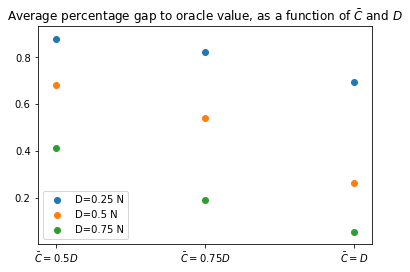
\includegraphics[scale=0.5]{simplot}
\caption{Percentage gap to oracle value ($\frac{ V(\pi^*) - V(\hat \pi, \bar{C})}{V(\pi^*) }$), under different deployment and contamination budgets. N=500, and 100 simulations for every parameter combination.}
\end{center}
\end{figure}


%\bpf

%which characterize the change in the optimal objective function value as a function of the perturbation to the coefficient vector $c$ of the LP, $|| \Delta c|| $.
%
%Suppose $||c(\Gamma) - c(\hat{\Gamma})|| \leq \delta$, then
%
%$$ R \leq K = \delta \frac{ \max \{ \sqrt{n+D^2}, || \Gamma^T X || \} }{ \sqrt{n+1} } \frac{ \sqrt{n+D^2} }{\sqrt{n+1} - \delta } $$
%
%where $|| \cdot ||$ refers to the 2-norm.
%
%$ || (\hat{\Gamma} - \Gamma)^T X || = \delta $
%

% Hence, we obtain
%$$ R \leq  || \Delta c || \frac{ ||d ||  }{ dist(d, Pri\emptyset) } \frac{||b||}{dist(d, Dual\emptyset)- || \Delta c || }. $$
%
%First, we note that the norm of the LP instance $d$ is given by the expression:
%
%$$||d ||  = \max \{ ||A || , ||b || , ||c ||  \} = \max \{ \sqrt{n+1}, \sqrt{n+D^2}, || \Gamma^T X || \} . $$
%
%Then, we refer to Corollary 2.9 of \cite{pena2003characterization} for an equivalent characterization of the distance to the primal infeasibility region in terms of the condition number of the coefficient matrix $A$ of the LP. 
%
%\begin{lem}[\cite{pena2003characterization} Corollary 2.9]
%For any given $A$, the distance to primal infeasibility, $dist(d_P, Pri\emptyset)$, is equal to
%\begin{align*}
%\rho(d_P) = \sup \{ \epsilon : ||y|| \leq \epsilon \Rightarrow y \in \{ Ax: x \geq 0, ||x|| \leq 1 \}  \},
%\end{align*}
%where $d_P = (A, b)$.
%\end{lem}
%
%Hence, we compute the condition number of $A$ as the largest singular value of the matrix $A$. That is, we have
%\begin{align*}
%\rho(d_P) = || A ||_2 = \sigma_{max} (A) = \sqrt{n+1}.
%\end{align*}
%
%Similarly, we can show that the distance to the dual infeasible region is given by the largest singular value of the transpose of the coefficient matrix $A^T$, i.e., $\rho(d_D) = || A^T ||_2 =  \sigma_{max} (A^T) = \sigma_{max} (A) $.
%
%Finally, we use the observation that the perturbation to the coefficient vector is smaller than $\delta$. Therefore, we can conclude that regret is upper bounded by
%
%$$ K = \delta \frac{ \max \{ \sqrt{n+1}, \sqrt{n+D^2}, || \Gamma^T X || \} }{ \sqrt{n+1} } \frac{ \sqrt{n+D^2} }{\sqrt{n+1} - \delta } $$.
%
%\begin{algorithm}
%    \caption{Contamination-aware sequential experimentation}
%    \label{cmu_sampling}
%    \begin{algorithmic}[] % The number tells where the line numbering should start
%        \Procedure{Calculate value}{Target, X (Matrix), Treated Nodes (Set), Exposed Nodes (Set)} 
%            \If{$ Target \in Treated Nodes$} \State \textbf{return} 0
%            \Else
%            \State $NewExposedNodes\gets Neighbors(Target) \cup ExposedNodes$
%            \State $Cost \gets |Neighbors(Target) \setminus ExposedNodes|$
%            \State $X_{E} \gets X[ExposedNodes]$
%            \State $X_{N} \gets X[NewExposedNodes]$            
%            \State $InformationGain \gets tr( (X_{E} X_{E} ^T) ^ {-1} ) - tr( (X_{N} X_{N} ^T) ^ {-1} )$
%            \State $Value \gets InformationGain/Cost$
%            \State \textbf{return} $Value$
%            \EndIf
%        \EndProcedure
%        \\\hrulefill
%        \Function{Sampling Path}{A (Matrix), $\bar{C}$ (Contamination Budget), X (Matrix)} 
%            \State $Path \gets [ ]$
%            \State $Cost \gets 0$
%            \State $Treated Nodes \gets \emptyset$
%            \State $Exposed Nodes \gets \emptyset$
%            \While{$Cost < \bar{C}$}
%                \State $a \gets b$
%                \State $b \gets r$
%                \State $r \gets a \bmod b$
%            \EndWhile\label{euclidendwhile}
%            \State \textbf{return} $b$
%        \EndFunction
%      \end{algorithmic}
%\end{algorithm}
%\begin{algorithm}
%    \caption{Calculate the value of experimenting on a node}
%    \begin{algorithmic}[1] % The number tells where the line numbering should start
%                \Procedure{Calculate value}{Target, X (Matrix), Treated Nodes (Set), Exposed Nodes (Set)} 
%            \If{$ Target \in Treated Nodes$} \State \textbf{return} 0
%            \Else
%            \State $NewExposedNodes\gets Neighbors(Target) \cup ExposedNodes$
%            \State $Cost \gets |UnexposedNeighbors|$
%            \State $X_{E} \gets X[ExposedNodes]$
%            \State $X_{N} \gets X[NewExposedNodes]$            
%            \State $InformationGain \gets tr( (X_{E} X_{E} ^T) ^ {-1} ) - tr( (X_{N} X_{N} ^T) ^ {-1} )$
%            \State $Value \gets InformationGain/Cost$
%            \State \textbf{return} $Value$
%            \EndIf
%        \EndProcedure
%    \end{algorithmic}
%\end{algorithm}

%\bibliographystyle{plain}
%\bibliography{references.bib}

\end{document}